\section{Anwendungsentwicklung mit Webtechnologien}

Die Sensorverwaltungsanwendung von Dryad wird mithilfe von Webtechnologien (html, css, javascript) und zahlreichen Tools entwickelt, um eine Webanwendung zu erstellen, die auf mehreren Plattformen (Browser, ios, Android) läuft und dabei nur einen einzigen Quellcode hat.
Es wurde beschlossen, dass die erste Version der Anwendung eine Single Page Application (SPA) sein sollte.
Derzeit gibt es viele Tools, die das Erstellen einer SPA erleichtern. Innerhalb von Cloud-Team von Dryad wurde beschlossen, die folgenden zu verwenden:

\subsection{Single Page Application (SPA)}

Eine Single Page Application ist ein Website-Design-Ansatz, bei dem der Inhalt jeder neuen Seite nicht durch das Laden neuer HTML-Seiten, sondern dynamisch durch die Fähigkeit von JavaScript, die \ac{DOM}-Elemente auf der bestehenden Seite selbst zu manipulieren, generiert wird.

\begin{figure}[h]
  \centering
  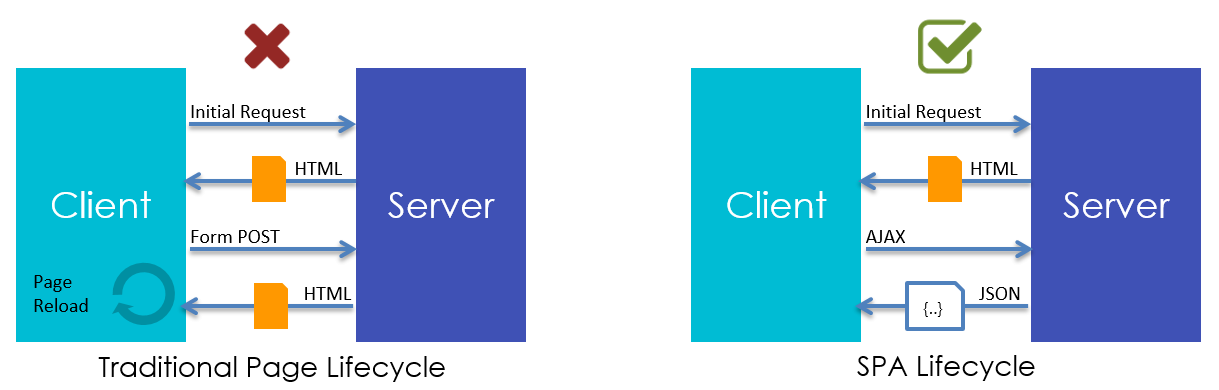
\includegraphics[width=\textwidth]{spa}
  \caption{https://www.tothenew.com/blog/optimization-of-angularjs-single-page-applications-for-web-crawlers/}
  \label{fig:spa}
\end{figure}

\textbf{Pros:}

\begin{itemize}
  \item Die traditionellen HTML-Seiten nehmen beim Hin- und Herbewegen zum Server viel Zeit in Anspruch. Dies erforderte das Nachladen der großen Menge ähnlicher Daten, während das neue SPA die Notwendigkeit der Kommunikation mit HTML-Tags zum Server mildert. SPA lädt nur einmal mit den HTML-Tags, während die nächsten Anfragen auf das teilweise Laden der Seite mittels AJAX und JSON erfolgen. Dies führt zu einer Einsparung von Bandbreite.
  \item Die SPA-Seite wird schneller geladen und benötigt aufgrund der geringeren Datentransaktion weniger Bandbreite. Das Seitendesign und UX werden besser und funktionieren erstaunlich gut mit den langsamen Verbindungen.
\end{itemize}

\textbf{Cons:}

\begin{itemize}
  \item Die traditionellen HTML-Seiten sind gut für den SEO, während die SPA schwer von den Benutzern gecrawlt werden kann, weil die Webcrawler nicht wissen, wie sie mit dem Javascript umgehen sollen. Die Lösung besteht darin, die roboterspezifische HTML-Seite zu kodieren, was wiederum zu Wartungsproblemen führen kann.
  \item Manchmal braucht die SPA viel Zeit, um das Bündel aus CSS und Javascript zu laden, was das erste Laden der Seite verzögert.
\end{itemize}

\subsection{TypeScript}

Die Entwicklung einer Webanwendung kommt heutzutage ohne Javascript kaum noch aus. Die Hegemonie dieser Sprache wird nicht mehr angezweifelt, und ihre Gemeinschaft ist eine der wichtigsten in der Welt der Webentwicklung, was sicherlich auf ihre inhärente Flexibilität zurückzuführen ist. Es hat jedoch einige Einschränkungen, wenn es um die Entwicklung komplexer Anwendungen geht, und aus diesem Grund kommt TypeScript ins Spiel.\cite{tsEssential}

\href{https://www.typescriptlang.org/}{TypeScript}\footnote{https://www.typescriptlang.org/} ist eine Programmiersprache, die von Microsoft im Jahr 2012 entwickelt wurde. Sein Hauptanliegen ist es, die Produktivität der komplexen Anwendungsentwicklung zu verbessern.

Es handelt sich um eine Open-Source-Sprache, die als höhere Schicht von Javascript entwickelt wurde. Jeder in Javascript gültige Code ist auch in TypeScript gültig. Die Sprache führt jedoch optionale Funktionen wie Typisierung oder objektorientierte Programmierung ein. Um diese Funktionen nutzen zu können, ist keine Bibliothek erforderlich, aber nur das Tool für die TypeScript-Kompilierung. Somit wird der ausgeführte Code ein Javascript-Äquivalent des kompilierten TypeScript-Codes sein.

Dieser Sicherheitstyp hat ihn bei Javascript-Entwicklern sehr beliebt gemacht, wie die
\href{https://survey.stackoverflow.co/2022/\#most-loved-dreaded-and-wanted-language-want}{Stackoverflow Survey 2022}\footnote{https://survey.stackoverflow.co/2022/\#most-loved-dreaded-and-wanted-language-want}
beweist:

\begin{figure}[h]
  \centering
  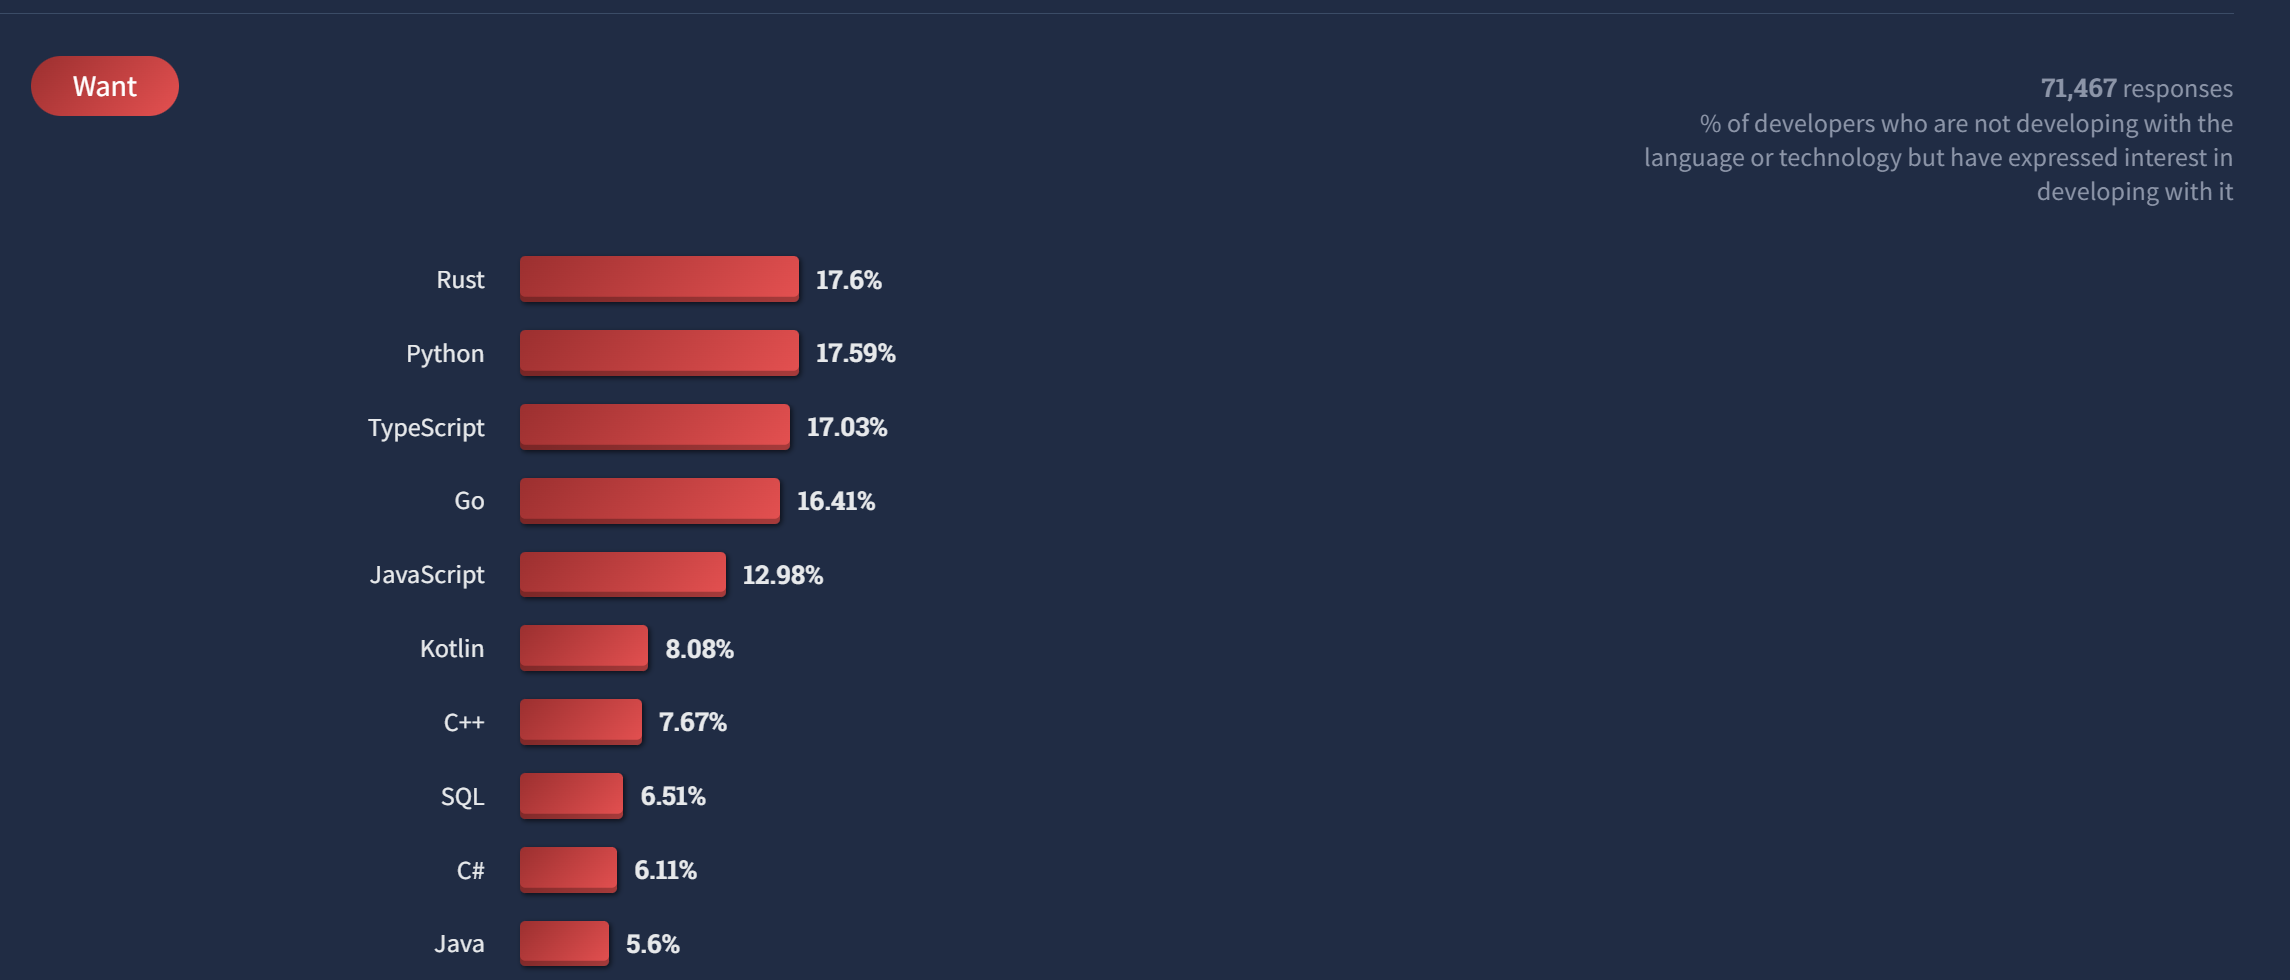
\includegraphics[width=\textwidth]{loved_programming_languages}
  \caption{Liste der beliebtesten Programmier-, Skript- und Auszeichnungssprachen im Jahr 2022}
  \label{fig:spa}
\end{figure}

\subsection{Webpack}
\href{https://github.com/webpack/webpack}{Webpack}\footnote{https://github.com/webpack/webpack} ist ein Modul-Bündler.
Sein Hauptzweck besteht darin, JavaScript-Dateien für die Verwendung in einem Browser zu bündeln, aber es ist auch in der Lage, so gut wie jede Ressource oder jedes Asset zu transformieren, zu bündeln oder zu {paketieren}\footnote{Offizielle Webpack-Dokumentation: \href{https://github.com/webpack/webpack\#webpack}{https://github.com/webpack/webpack\#webpack}}.

Es gibt viele verschiedene Bündler wie \href{https://parceljs.org/}{Parceljs}\footnote{https://parceljs.org/}, \href{https://github.com/rollup/rollup}{Rollupjs}\footnote{https://github.com/rollup/rollup} oder \href{https://github.com/browserify/browserify}{Browserify}\footnote{https://github.com/browserify/browserify}.
Das von uns verwendete Web-Framework (das im nächsten Abschnitt vorgestellt wird) kommt jedoch fertig mit einer webpack-Konfiguration.
So wird webpack neben seiner Reife, seinen zahlreichen Plug-ins und seiner umfangreichen Konfiguration auch für den Aufbau unserer Javascript-Anwendung verwendet.

\subsection{Angular}
Mit Javascript können wir ein HTML DOM leicht manipulieren. Das Hinzufügen, Ändern oder Löschen eines Node zur Laufzeit, ohne die Seite neu zu laden, bietet dem Benutzer eine sehr dynamische und leichte Schnittstelle, die dem ähnelt, was er in einer nativen Anwendung sehen kann.

Leider kann die Entwicklung einer Webanwendung allein mithilfe von Javascript sehr viel Zeit in Anspruch nehmen und schwer skalierbar werden.
Aus diesem Grund haben sehr marktführende Unternehmen wie Google oder Facebook ihr Javascript-Framework entwickelt, um dynamische Schnittstellen einfach zu erstellen.

Ein Framework ist eine semi-vollständige Applikation. Es stellt für Applikationen eine wiederverwendbare, gemeinsame Struktur zur Verfügung.
Die Entwickler bauen das Framework in ihre eigene Applikation ein und erweitern es derart, dass es ihren spezifischen Anforderungen entspricht.
Frameworks unterscheiden sich von Toolkits dahingehend, dass sie eine kohärente Struktur zur Verfügung stellen, anstatt einer einfachen Menge von Hilfsklassen\cite{DesigningReusableClasses}.

Einige der beliebtesten sind \href{https://github.com/facebook/react/}{React}\footnote{https://github.com/facebook/react/} von Facebook,
\href{https://github.com/facebook/react/}{Angular}\footnote{https://github.com/angular/angular} von Google und
\href{https://github.com/facebook/react/}{Vue}\footnote{https://github.com/vuejs/vue}.

\begin{figure}[h]
  \centering
  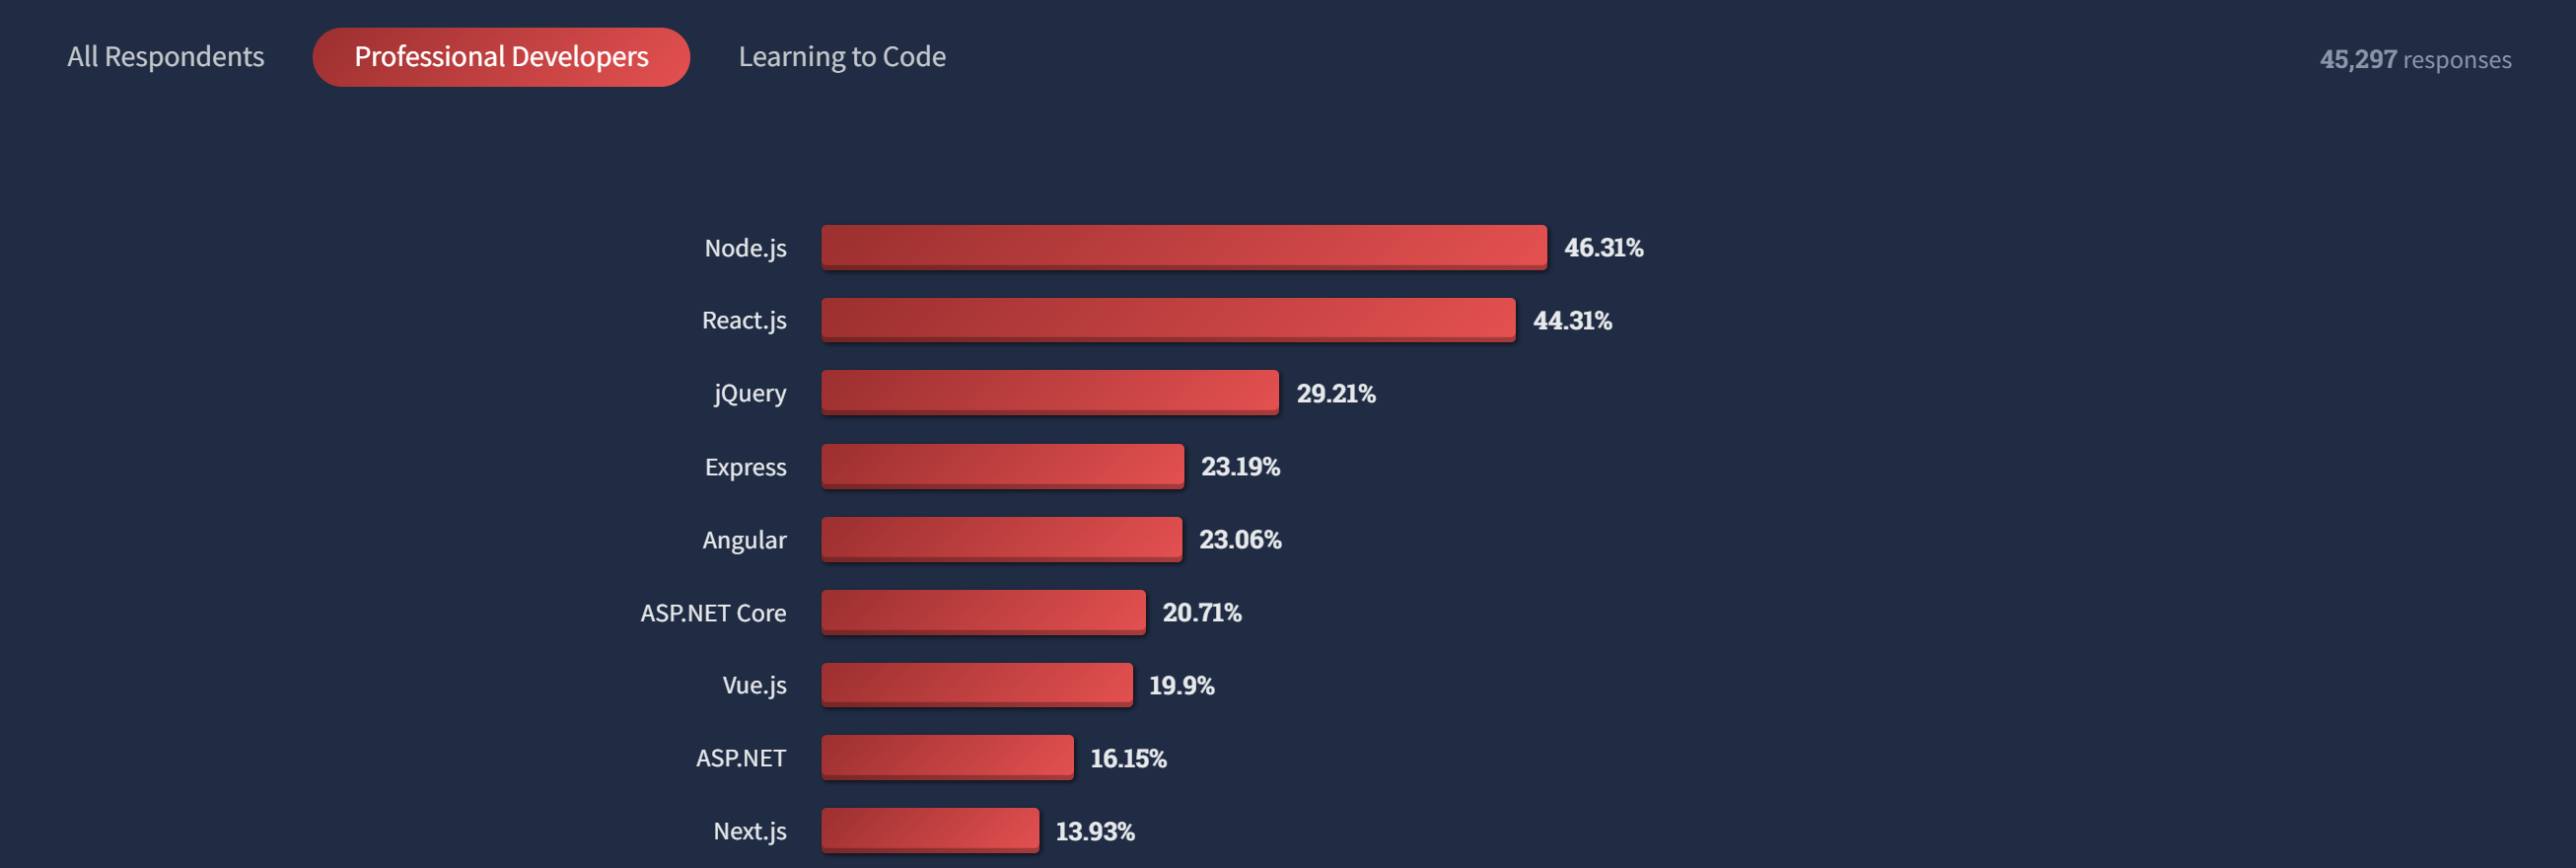
\includegraphics[width=\textwidth]{loved_frameworks}
  \caption{Stackoverflow Survey 2022: Beliebteste Web-Frameworks}
\end{figure}

Angular wurde aufgrund seines umfassenden Designs, seiner großen Nutzergemeinde und der Tatsache, dass das Team bereits über fundierte Kenntnisse in diesem Tool verfügte, als Framework ausgewählt.

\subsection{Npm}
Es ist derzeit undenkbar, eine Webapplikation von Grund auf neu zu entwickeln.
Es gibt eine Vielzahl von Open-Source-Bibliotheken, die von verschiedenen Entwicklern entwickelt wurden und mit denen unsere Anwendung schnell und einfach erstellen werden kann.
Deshalb ist es notwendig, ein Tool zu benutzen, um die verschiedenen Bibliotheken, die verwendet werden, zu organisieren.

\ac{NPM} ist das Zentrum der gemeinsamen Nutzung von JavaScript-Code und mit mehr als einer Million Paketen und 11 Millionen Entwickler weltweit die größte Software-Registry der Welt\footnote{npmjs offizielle Website: \href{https://www.npmjs.com/}{https://www.npmjs.com/}}.
Aufgrund dieses guten Renommees beschloss das Team, NPM zur Verwaltung der verschiedenen Bibliotheken einzusetzen.

\subsection{SASS}
Angular erlaubt es, das DOM einer Webanwendung leicht zu manipulieren, bleibt nur noch, sie zu stylen.
Es wird dafür der Stylesheet-Kernsprachen des World Wide Webs verwenden, \ac{CSS}.

Leider kann CSS schnell überflüssig und schwierig zu handhaben werden, wenn es darum geht, mehrere Dutzend Elemente gleichzeitig zu bearbeiten.
Um dieses Problem zu überwinden, wurde der CSS-Präprozessor \ac{SASS} geschaffen, der die Verwendung von Variablen, Schleifen und Funktionen erlaubt, die in CSS umgesetzt werden.

Die folgende Abbildung zeigt die gleiche Style-Deklaration mit CSS und SASS:

\begin{table}[H]
  \begin{tabular}{c c}
    CSS & SASS \\
    \begin{lstlisting}[language=css]
  ul {
    background-color: red;
  }

  ul.hide {
    opacity: 0;
  }

  ul.hide li {
    text-decoration: underline;
  }
      \end{lstlisting}
        &
    \begin{lstlisting}[language=css]
  ul {
    background-color: red;

    &.hide {
      opacity: 0;

      li {
        text-decoration: underline;
      }
    }
  }
            \end{lstlisting}
  \end{tabular}
  \caption{Beispiel für die Deklaration von Styles in CSS und SASS }
\end{table}

Es wurde daher beschlossen, diesen css-Prozessor im Projekt zu verwenden. Außerdem bietet Angular eine bereits fertige Sass-Kompilation an.

\subsection{Angular Routing}

Der Antrag wird also von einer einzigen Seite generiert, was aber nicht bedeutet, dass ein Wechsel der URLs nicht möglich ist.
Tatsächlich kann eine SPA dank Javascript auf verschiedenen URLs laufen.
Angular bringt ein eigenes Routing-System namens Angular Routing\footnote{https://angular.io/guide/routing-overview} mit, das es ermöglicht, bestimmte Komponenten auf der Grundlage der URL anzuzeigen. Das Projekt wird diese Lösung verwenden, um das Routing der Anwendung zu verwalten.

